\documentclass[twocolumn,a4paper,10pt,english]{article}

\usepackage{graphicx}
\usepackage[latin1]{inputenc}
\usepackage{fancyhdr}
\usepackage{geometry}
\usepackage[english]{babel}
\usepackage{amsmath}
\usepackage[breaklinks]{hyperref}
\usepackage[small,hang]{caption}
\renewcommand{\captionfont}{\it \footnotesize}
\renewcommand{\captionlabelfont}{\it \bf \footnotesize}
	\hypersetup{
    colorlinks,
    citecolor=black,
    filecolor=black,
    linkcolor=black,
    urlcolor=blue
	}
\usepackage{float}
\graphicspath{{./images/}}
\DeclareMathOperator{\sign}{sign}
\geometry{a4paper,tmargin=3.7cm,bmargin=2cm,lmargin=1.5cm,rmargin=1.5cm,headheight=2.2cm,headsep=0.5cm,footskip=0.5cm}
\columnsep=0.6cm
\setlength\parindent{0pt}

\newcommand{\dd}[2]{\frac{\partial #1}{\partial #2}}


\fancypagestyle{plain}{
\lhead{
\includegraphics[height=15mm]{VL_SUPAERO_300_cmjn}}
\rhead{M. Pioli\\
J. Mas Colomer\\
J. Morlier\\
PZT modeling in OpenNastran95 for scaled aircraft in aeroelastic similarity}  
\cfoot{}
\lfoot{\small \copyright Institut Sup\'{e}rieur de l'A\'{e}ronautique et de l'Espace}
\renewcommand{\headrulewidth}{0.4pt}
}
\rfoot{\thepage}

\title{\textbf{\sc PZT modeling in OpenNastran95 for scaled aircraft in aeroelastic similarity\vspace{-0.5cm}}}
\author{
	\textsc{Michele Pioli}\vspace{-0.5cm}\\
	\textsc{Joan Mas Colomer, PhD candidate}\vspace{-0.5cm}\\
	\textsc{Prof. Joseph Morlier}
}

\date{}
\pagestyle{plain}

\def\arraystretch{2.5}
\begin{document}

\thispagestyle{plain}

\maketitle


\begin{abstract}
    To overcome the lack of piezoelectric elements in OpenNastran95, two ways of modeling their effect are investigated. A thermal analogy to represent the piezoelectric expansion/contraction and an actuation modeling through applied bending moments have been implemented in OpenNastran95. The application of these tools is discussed using a cantilever aluminum beam with a surface mounted piezoelectric actuator as a sample problem.\\
	A Python code used to modify the Nastran input file by filling a template with the materials properties and voltage loads on PZT actuators is then presented.\\
	The OpenNastran95 input files and the Python code are provided.
	Analyses results are generated in terms of nodal displacements due to the input voltage applied to the actuator.\\
    
    \textbf{Keywords: } Structural Mechanics; Smart Structure; Piezoelectric; OpenNastran95; Finite Element Method 
\end{abstract}

\section{Introduction}
	        
    \subsection{Motivations}
    There are many structures which can benefit from the control offered by piezoelectric materials: using piezoelectric actuators and sensors to form self-controlling and self-monitoring systems to improve performance of aircraft and space structures has attracted interest in the research community.\\
     Piezoelectric materials respond elastically to an applied electric potential gradient. The ability to generate an electrical response from an applied mechanical load, and vice versa, allows piezoceramic actuators and sensors to be used as active structural members in smart structures. \\
     This paper focuses on the modeling of surface-bonded piezo-actuators through OpenNastran95. The main interest is to add their thickness and applied voltage to the design variables set used to perform a multidisciplinary optimization of a scaled aircraft in aeroelastic similarity through the framework \textit{OpenMDAO}.
    
        \subsubsection{Aeroelastic Stability}
            The study of aeroelasticty can be classified into two main branches: static aeroelasticity and dynamic aeroelasticity.\\
            In static aeroelasticity, "fast" dynamics of structure and aerodynamics are neglected and it focuses on "slow" effect of fluid-structure interaction: no inertia forces due to structural deformation are taken into account, only rigid body motion inertia forces are accounted for. In order to get a target structural in-flight static deformation, in addition to the classical variables (such as materials, thicknesses, shapes, masses etc...), the placement of piezoelectric patches might be useful. Actually, the patch thickness and the voltage applied to it can be used as two extra degree of freedom for the scope.\\
            When it comes to dynamic aeroelasticity, $flutter$ is certainly the main phenomenon. From the physical standpoint, it consists of divergent oscillations of an elastic structure subjected to an air flow: the damping of structural modes goes to zero in correspondence of a certain velocity. Mathematically, the $flutter$ analysis is the  study of a linearized system where the eigenvalues behavior is observed: the real part of at least one mechanical pole vanishes because of aerodynamics. It goes to the complex plane right-half, causing a dynamic instability. There are both passive and active methods to avoid the $flutter$ occurrence. A proper structural design, paying attention to stiffness and mass properties, or the use of flight control system and aerodynamic surfaces for an active flutter suppression are methods widely spread over the aeronautical industry. The adoption of piezoelectric patches integrated in the structure might represent another technique to tackle this problem.
            
            
        \subsubsection{Wing modal tuning for scaled aircraft}
	        The aircraft aeroelastic behavior is strictly related to its modal response; therefore, it is convenient to design the aircraft such that its natural frequencies guarantee the aircraft aeroelastic stability within the flight envelope. There are several techniques which might be applied for the scope of modal tuning, some of them act passively on the structure, such as the concentrated masses, and others actively, such as the piezoelectric patches subjected to an external voltage across the electrodes. 
	        When it comes to a scaled aircraft in aeroelastic similarity, we aim at getting the same vibrational modes, frequencies and flutter velocity of the reference aircraft. Again, the piezoelectric patch thickness and voltage might be used as additional variables for the scope. 
            
            
            
        \subsubsection{Piezoelectric materials overview}
            Piezoelectric materials undergo a deformation when a voltage is applied. Conversely, a voltage is produced when a piezoelectric material is deformed.
            Actually, the constitutive law of piezoelectric materials implies an electro-structural interaction which describe this coupling. In particular, under the hypothesis of linear behavior, it is possible to write the law in a practical way, obtained recasting what is written in \cite{c1}:
            \begin{equation}
            \begin{cases}
            \epsilon = E_{\epsilon\sigma}\sigma + E_{\epsilon e}e & \text{inverse effect: actuators}\\d = E_{d\sigma}\sigma + E_{de}e & \text{direct effect: sensors}
            \end{cases}
            \label{con_law}
            \end{equation}
            where $e$ is the electric field (remind: $e=\nabla V$, where $V$ is the voltage), $d$ the dielectric field, $\sigma$ and $\epsilon$ are respectively the stress and the strain of the material. \\
            Furthermore, there are some symmetry properties: $E_{\sigma\epsilon}=E_{\sigma\epsilon}^T$, $E_{de}=E_{de}^T$.\\
            The matrix $E_{de}$ is the dielectric constants matrix, while $E_{\epsilon e}$, is piezoelectric constants matrix.\\
            $E_{\alpha\beta}$ are sparse matrices: the piezoelectric effect, both direct and inverse, does not involve all the directions. We can distinguish two main effects: the co-directional one in case the deformation is in the same direction as the electric field $e$ and the transversal one when it is transversal to $e$.\\
            By inverting the relations \ref{con_law}, it is possible to write:
            \begin{equation}
            \begin{cases}
            \sigma = E_{\epsilon\sigma}^{-1}\epsilon + E_{\epsilon\sigma}^{-1}E_{\epsilon e}e \\
            d = E_{d\sigma} (E_{\epsilon\sigma}^{-1}\epsilon + E_{\epsilon\sigma}^{-1}E_{\epsilon e}e) + E_{de}e 
            \end{cases}
            \label{inv_con_law}	
            \end{equation}
            Then, by renaming the matrices, we get the elastic/electric constitutive law in a form that will be useful in the following:
            \begin{equation}
            \begin{cases}
            \sigma = D\epsilon -Ee \\
            d = E^T \epsilon + \mathcal{E} e 
            \end{cases}
            \label{useful_con_law}	
            \end{equation}
            In this paper, the main interest lies in the first equation of \ref{con_law}: the one describing the inverse effect. It can be noticed that by  applying an electric field to the material, a strain is generated.
            $E_{\epsilon e}$, the piezoelectric constants matrix, can be written in the form:
            
            \[
            E_{\epsilon e}=
            \begin{bmatrix}
            0 & 0 & d_{31}\\ 	0 & 0 & d_{32}\\ 	0 & 0 & d_{33}\\
            0 & d_{24} & 0\\    d_{15} & 0 & 0\\    0 & 0 & 0
            \end{bmatrix}
            \]
            where coefficients are written this way to comply with the conventional notation in piezoelectric materials where the $z$-direction (3-direction) is aligned with the "poled" direction of the material, as shown in Fig.\ref{fig:pzt}.
            \begin{figure}[htp]
            	\centering
            	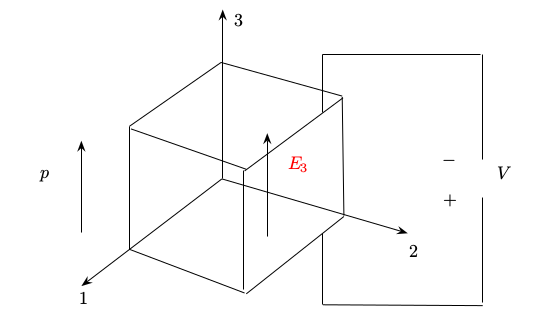
\includegraphics[width=0.7\linewidth]{images/pzt31.png}
            	\caption{PZT reference system}
            	\label{fig:pzt}
            \end{figure}\\
            Piezoelectric materials can be distinguished in two main categories, as shown in Tab.\ref{tab:piezo}.
            \begin{table}[H]
            	\begin{tabular}{|c|c|c|}      
            		\hline      		
            		\textbf{Type} & \textbf{Coefficients} & \textbf{Use}\\ 
            		\hline           		
            		PZT (Ceramic) & $d_{31}=d_{32}, d_{15}=d_{24}$ & Actuators \\
            		\hline
            		PVDF (Polymeric) & $d_{15}=d_{24}=0$ & Sensors \\
            		\hline
            	\end{tabular}
            	\caption{Piezoelectric types}
            	\label{tab:piezo}
            \end{table}
             When it comes to PZT patches, the ones used in the following, the predominant effect is $d_{31}$ (or, equivalently $d_{32}$), therefore:
            \begin{equation*}
            \epsilon_{11}=d_{31}e_3=d_{31}\dfrac{V}{h_p}
            \end{equation*}
            where $h_p$ the thickness of the patch.\\
            By using the form \ref{useful_con_law} of the constitutive law, reminding that it can be written:
             \begin{equation}
             \begin{cases}
             e=grad(V) \\
             \epsilon = Bu 
             \end{cases}	
             \end{equation}
             therefore
              \begin{equation}
              \begin{cases}
              \sigma = D\epsilon -E grad(V) \\
              d = E^T \epsilon + \mathcal{E} grad(V) 
              \end{cases}
              \label{substituted}	
              \end{equation}
              The first equation of \ref{substituted} leads to a change in the stiffness matrix. Written in the weak form is:
              \begin{equation}
              	\int_{\mathcal{V}} \delta \epsilon^T \sigma d\mathcal{V} = \int_{\mathcal{V}} \delta \epsilon^T D \epsilon d\mathcal{V}-\int_{\mathcal{V}} \delta \epsilon^T E grad(V) d\mathcal{V}
              \end{equation}
				Remembering that the work is the electrical charge times the potential difference and that the first Maxwell equation states:
				\begin{equation}
					\nabla \cdot d = \rho_F
				\end{equation}
				where $\rho_F$ is the free charge, then:
				\begin{equation}
				\int_{\mathcal{V}} \delta V^T div(d) d\mathcal{V}=\int_{\mathcal{V}} \delta V^T \rho_F d\mathcal{V}	
				\end{equation}
				integrating by parts:
				\begin{equation}
						-\int_{\mathcal{V}} \delta grad(V)^T d~ d\mathcal{V}+\int_{\mathcal{V}} \delta V^T d\cdot n~ d\mathcal{S}=\int_{\mathcal{V}} \delta V^T \rho_F d\mathcal{V}
				\end{equation}
				The second term on the left-hand side is the natural boundary condition, i.e. the superficial charge ($\rho_S$), which can be taken to the right-hand side:
				\begin{equation}
				-\int_{\mathcal{V}} \delta grad(V)^T d~ d\mathcal{V}=\int_{\mathcal{V}} \delta V^T \rho^* d\mathcal{V}
				\end{equation}	
				Now, the expression of $d$ (see second Eq. of \ref{substituted}) can be introduced in the equation:
				\begin{equation}
					-\int_{\mathcal{V}} \delta grad(V)^T (E^T \epsilon + \mathcal{E} grad(V))~ d\mathcal{V}=\int_{\mathcal{V}} \delta V^T \rho^* d\mathcal{V}
				\end{equation}
				It is possible to rewrite the last equation this way:
					\begin{equation}
					\int_{\mathcal{V}} \delta \nabla V^T E^T Bu~d\mathcal{V}+\int_{\mathcal{V}} \delta \nabla V^T \mathcal{E} \nabla V~ d\mathcal{V}= \int_{\mathcal{V}} \delta V^T \rho_S d\mathcal{V}
					\end{equation}
					where the free charge has been put to zero ($\rho_F=0$) and the strain has been substituted by its discretization.
					Introducing the following assumption for the electrical potential:
					\begin{equation}
						V(x,t)=N_V(x)q_V(t)
					\end{equation}
					and, therefore
					\begin{equation}
					grad~V=grad\{N_V\}q_V
					\end{equation}
					the two equations become:
					\begin{equation}\begin{split}
					\delta u^T \int_{\mathcal{V}}  &B^TDB~d\mathcal{V}~u+\\
					&-\delta u^T \int_{\mathcal{V}}  B^TEgrad\{N_V\}~d\mathcal{V}~q_V=\delta u^TF
					\end{split}
					\end{equation}
					and
					\begin{equation}\begin{split}
						&\delta q_V^T\int_{\mathcal{V}} \nabla\{N_V\}^T E^T B~d\mathcal{V}~u+\\
						&+\delta q_V^T\int_{\mathcal{V}} \nabla\{N_V\} ^T \mathcal{E} \nabla\{N_V\}~ d\mathcal{V}~q_V=
						 \delta q_V^T\int_{\mathcal{V}} \{N_V\}V^T \rho_S d\mathcal{V}	
					\end{split}
					\end{equation}
					where the first equation expresses the stiffness variation term.
					Actually, because of the virtual displacements arbitrariness, the strong form system is:
					\begin{equation}
						\begin{cases}
						M\ddot{u}+Ku-K_{uV}q_V=F \\
						S_{du}u+C_eq_V=\rho_{ext} 
						\end{cases}
					\end{equation}
					where $S_{du}$ is the structural charge matrix and $C_e$ is the capacity matrix.
					The coupling term $S_{du}=\int_{\mathcal{V}} \nabla\{N_V\}^T E^T B~d\mathcal{V}$ can be transformed to the modal space through the expansion $u=Uq$ (the potential consists of few developing terms so it is possible not to condense it in the modal form). Hence:
					\begin{equation}
						\int_{\mathcal{V}} \nabla\{N_V\}^T E^T B~d\mathcal{V}~U
					\end{equation}
					It is now evident that the generalized modal outputs depend on the piezoelectric material distribution. It will be possible to design the piezoelectric material distribution in order to activate a mode rather than another one.\\ 
					\medskip
					\textbf{Observation.} Maxwell's equations:
					\begin{equation}
					\begin{cases}
					\nabla \cdot d=\rho_F \\
					\nabla \times e = -\frac{\partial b}{\partial t}\\
					\nabla \cdot b=0 \\
					\nabla \times h = j+\frac{\partial d}{\partial t}
					\end{cases}
					\end{equation}
					In case of time dependent dielectric field, an associated magnetic field will rise up and, as a consequence, an electromagnetic coupling.
					This effect will be neglected in what follows since the electromagnetic dynamics is residualized (static or quasi-static approach). Our interest lies in low frequencies. Assuming an electromagnetic waves propagation velocity of $300.000 km/s$, for frequencies up to some ten $kHz$ (already very high), the wave length is roughly $10 km$. In the structural systems dimensional scale, the quasi-steady approach is therefore appropriate. 
\section{Methodology}
    
    \subsection{PZT modeling through thermal deformation}
    
        According to \cite{c5}, the piezoelectric actuation effect can be modeled with the thermal expansion/contraction. The term related to strains induced by temperature appears on the right-hand-side of the Finite Element equation:
    
        \begin{equation}
            Thermal= \int_V [B]^T[D]\{\alpha\}(T)dV
        \end{equation}
        
        where $[B]$ is the shape functions derivatives matrix, $[D]$ the elastic constitutive matrix, $\{\alpha\}$ contains the thermal expansion coefficients, and $T = T^*-T_0$ is the applied temperature relative to reference, $T_0$.\\
        The piezoelectric term appearing in the FE equilibrium equation is the following:
        
        \begin{equation}
        	PZT= \int_V [B]^T[D][d](E)dV
        \end{equation}
	    
	   
        The thermal analogy to piezoelectric voltage actuation is immediate: the piezoelectric constant matrix $[d]$, with elements relating mechanical strain produced by an applied electric field, collapses to the CTE vector $\{\alpha\}$, with elements relating mechanical strain produced by a change in temperature. The electric field vector $(E)$ loses its role to the temperature scalar $(T)$. Hence:
        \begin{equation}
        {d_{31}}\frac{V}{h}\leftrightarrow \alpha T
        \end{equation}
        
         In case of simultaneous voltage and thermal loads, it is still possible to model the problem. In fact:
         \begin{equation}
         \epsilon_j=\alpha_j T+ d_{3j}\frac{V_3}{h}
         \end{equation}
         \begin{equation}
         \epsilon_j=CTE_j(T+\frac{d_{3j}}{CTE_j} \frac{V_3}{h})=CTE_jT_{eff}
         \end{equation}
        
        The simple thermal analogy has been adopted by \cite{c2}, where no real thermal loads are accounted for (only to represent the piezoelectric effect). There, a structure with piezoelectric actuator is modeled by using MSC/Nastran.	A cantilevered aluminum beam, Fig.\ref{fig:beam}, with one piezoelectric actuator bonded near the root as a sample problem is used in this study. 
        \begin{figure}[htp]
        	\centering
        	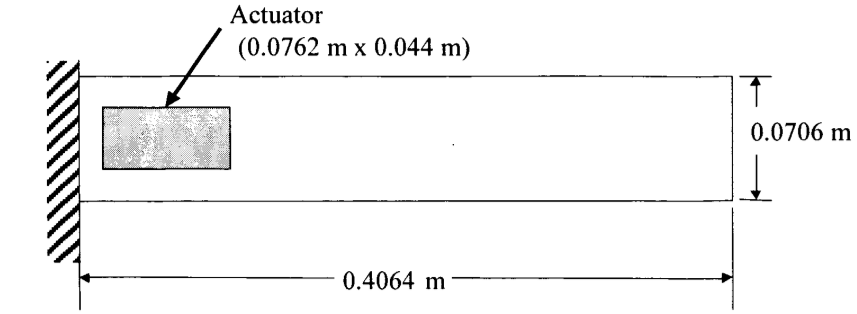
\includegraphics[width=0.6\linewidth]{images/nasa.png}
        	\caption{Cantilevered aluminum beam with piezoelectric actuator}
        	\label{fig:beam}
        \end{figure}\\
        Piezoelectric coefficients characterizing the actuator are input as thermal expansion coefficients $(CTE's)$ associated with standard elements. In this study the model treats both the actuator and the structures substrates as plies of an integrated laminated plate. PCOMP cards in MSC/NASTRAN are used to specify the properties of the composite lay-up and the applied voltage is modeled as a thermal load. TEMP cards identify the locations at which thermal loads (voltage) is applied.
	    Through MAT1 cards the 	non-zero thermal expansion coefficient is assigned to the patch while the $CTE$ in the remaining structure must be zero to ensure thermal expansion loads are generated only at the piezoelectric actuator locations. As mentioned above, the $CTE$ of the patch is computed this way:
	    \begin{equation}
	    	\alpha=\frac{d_{31}}{t}
	    \end{equation}
	    The first step of the analysis is the generation of Ritz vectors: static deflection vectors due to a thermal load equivalent to $1V$. Since one Ritz vector is required for each independently actuated piezo, in this case only one vector is computed.
	    Then, a general eigensolution combines the Ritz vectors with eigenvectors and
	    calculates the mass and stiffness matrices needed to assemble a reduced order model. Finally, MATLAB scripts are required to assemble the dynamic equations and generate frequency response functions (FRF) at the observation points: some nodes placed along the beam axis close to the tip are considered. The FRF of the tip displacement as a function of the PZT input voltage is reported in Fig. \ref{fig:frf}
	    \begin{figure}[htp]
	    	\centering
	    	%	\setlength\figureheight{2cm}
	    	%	\setlength\figurewidth{2cm}
	    	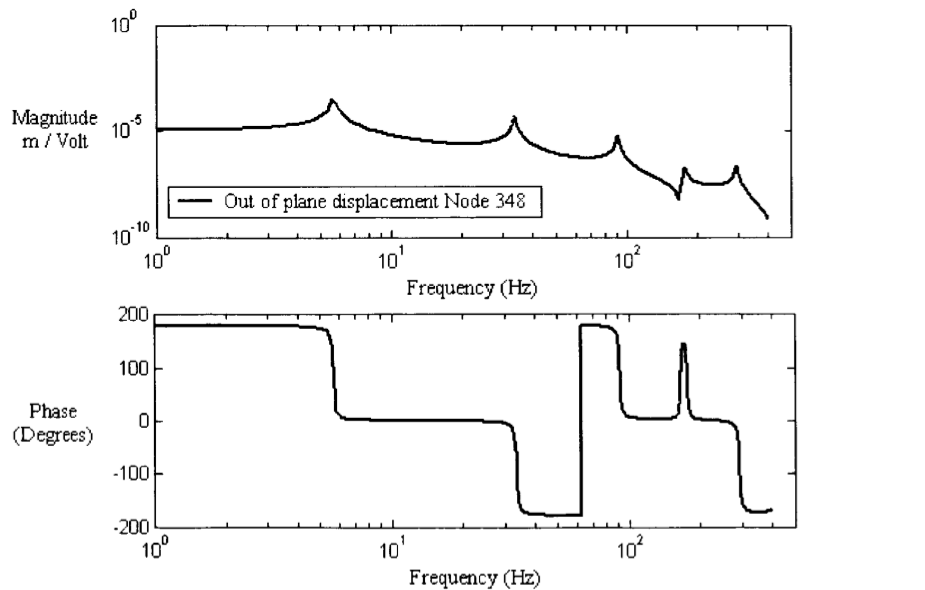
\includegraphics[width=0.6\linewidth]{images/frf.png}
	    	\caption{FRF of aluminum beam tip displacement as a function of piezoelectric actuator input voltage}
	    	\label{fig:frf}
	    \end{figure}\\ 
	    Some peaks can be observed in the magnitude plot: the PZT actuation is more effective in correspondence of certain frequencies.\\
	    Herein, the same sample problem has been reproduced using OpenNastran95 in order to get the static deformation of the beam. Both the PZT-5A and the PZT-5H have been modeled. The properties of the first one are reported in Tab.\ref{tab:5A}, while the ones of the PZT-5H in Tab.\ref{tab:5H}.
	    
	    \begin{table}[H]
	    	\footnotesize
	    	\def\arraystretch{1.2}
	    	\centering
	    	\begin{tabular}{|c|c|c|}
	    		\hline
	    		\textbf{Quantity} & \textbf{Symbol} & \textbf{Value} \\
	    		\hline
	    		Young's modulus & $E$ & $6.6\times10^4~MPa$  \\
	    		\hline
	    		Poisson ratio & $\nu$ & $0.31$ \\ 
	    		\hline
	    		Density &$\rho$ & $7.7\times10^{-9}~ton/mm^3$ \\
	    		\hline
	    		Piezoelectric coefficient & $d_{31}$ & $1.709\times10^{-7}$ \\
	    		\hline
	    		Patch thickness & $t$ & $0.203~mm$ \\
	    		\hline
	    		CTE & $\alpha=\frac{d_{31}}{t}$ & $8.42\times10^{-7}$ \\
	    		\hline
	    	\end{tabular}
	    	\caption{PZT-5A properties}
	    	\label{tab:5A}
	    \end{table}
		\begin{table}[H]
			\footnotesize
			\def\arraystretch{1.2}
			\centering
			\begin{tabular}{|c|c|c|}
				\hline
				\textbf{Quantity} & \textbf{Symbol} & \textbf{Value} \\
				\hline
				Young's modulus & $E$ & $6.061\times10^4~MPa$  \\
				\hline
				Poisson ratio & $\nu$ & $0.289$ \\ 
				\hline
				Density &$\rho$ & $7.5\times10^{-9}~ton/mm^3$ \\
				\hline
				Piezoelectric coefficient & $d_{31}$ & $2.74\times10^{-7}$ \\
				\hline
				Patch thickness & $t$ & $0.203~mm$ \\
				\hline
				CTE & $\alpha=\frac{d_{31}}{t}$ & $1.35\times10^{-6}$ \\
				\hline
			\end{tabular}
			\caption{PZT-5H properties}
			\label{tab:5H}
		\end{table}
		It can be noticed that the first one (PZT-5A) is stiffer than the second one (PZT-5H) and its piezo coefficient is lower: the displacements due to the same applied voltage will be smaller. \\
	    As far as the beam substrate is concerned, it is made of aluminum: its material properties, used to fill the MAT1 card, are reported in Tab.\ref{tab:Alu} 
	    	\begin{table}[H]
	    		\footnotesize
	    		\def\arraystretch{1.2}
	    		\centering
	    		\begin{tabular}{|c|c|c|}
	    			\hline
	    			\textbf{Quantity} & \textbf{Symbol} & \textbf{Value} \\
	    			\hline
	    			Young's modulus & $E$ & $7.2\times10^4~MPa$  \\
	    			\hline
	    			Poisson ratio & $\nu$ & $0.33$ \\ 
	    			\hline
	    			Density &$\rho$ & $2.758\times10^{-9}~ton/mm^3$ \\
	    			\hline
	    			Substrate thickness & $t$ & $1.016~mm$ \\
	    			\hline
	    			CTE & $\alpha$ & $0$ \\
	    			\hline
	    		\end{tabular}
	    		\caption{Aluminum properties}
	    		\label{tab:Alu}
	    	\end{table}
    	The $CTE$ is put to zero to ensure thermal expansion loads are generated only
    	at the piezoelectric actuator locations.\\
	    The geometrical dimensions are respectively $405\times70.56\times1.016~mm$ for the beam and $76\times39.2\times0.203~mm$ the patch. The mesh is composed by $450$ nodes and $396$ quadrilateral elements ($CQUAD4$). Along the transversal direction of the beam, there are $9$ elements of the same width ($7.84~mm$). The other elements' dimension, the one in the beam axis direction, is not always constant. In particular, the first two rows of elements starting from the root of the beam are smaller ($3~mm$) than the following ones ($9.5~mm$). This way, the boundary solution is "confined" and it does not involve the PZT patch. Actually, this one is placed exactly after the first two rows of elements, at $6~mm$ from the root. The OpenNastran95 input file is provided in the Appendix, except for the entire mesh. 
    \subsection{PZT modeling through applied moments}
	    In order to see how to model a PZT patch in a different way, the Virtual Work Principle has been applied to the same sample problem, a cantilever beam with a PZT actuator, as showed in Fig.\ref{fig:vwp}.\\
	    \begin{figure}[htp]
	    	\centering
	    	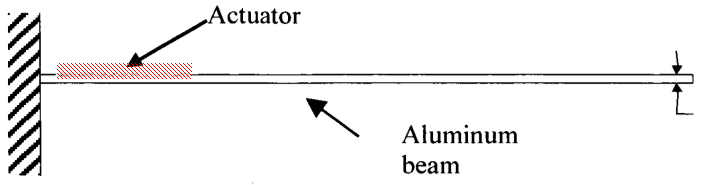
\includegraphics[width=0.6\linewidth]{images/vwp.jpg}
	    	\caption{Cantilever beam actuated by a piezoelectric patch}
	    	\label{fig:vwp}
	    \end{figure}\\
	    The Virtual Work Principle states:
	    \begin{equation}
	    \delta\mathcal{W}_D=\delta\mathcal{W}_E \Longrightarrow \int\delta\epsilon^T\sigma dV=-\int\delta v^T \rho\ddot{v}dV
	    \end{equation}
	    therefore, the internal deformation virtual work is equal to the external work due to inertia ($\delta v$ is the virtual displacement in the vertical direction $y$, $\rho$ is the material density).\\
	    Splitting the integrals on the beam volume and the PZT volume:
	    \begin{equation}\begin{split}
	    \int_{V_B}\delta\epsilon_B^T\sigma_B dV_B+&\int_{V_P}\delta\epsilon_P^T\sigma_P dV_P=\\
	    &-\int_{V_B}\delta v^T \rho_B\ddot{v}dV_B-\int_{V_P}\delta v^T \rho_P\ddot{v}dV_P
	    \label{virtual_developed}
	    \end{split}\end{equation}
	    We can easily notice that the first term can be rewritten in the following way:
	    \begin{equation}
	    	\int_{V_B}\delta\epsilon_B^T\sigma_B dV_B=\int_{V_B}\delta v^{''}EJv{''}dV_B
	    \end{equation}
	    only accounting for the deformation energy associated to bending. The product $EJ$ actually represents the bending stiffness of the beam.\\
	    Focusing on the second term of \eqref{virtual_developed}, the deformation internal virtual work of the PZT, we can rewrite it this way:
	    \begin{equation}
	    \int_{x_1}^{x_2}\int_{A_P}\delta\epsilon_{x_P}^T\sigma_{x_P} dA_P dx
	    \end{equation}
	    separating the integral on the patch section and on its $x$-axis.
	    By recasting the first equation of the constitutive law, keeping in mind that $\epsilon_{11}=d_{31}e_3=d_{31}\dfrac{V}{t_{pzt}}$ for strain due to voltage, we get the following expression for the stress in the PZT:
	    \begin{equation}
	    \sigma_{x_P}=E_p\epsilon_{x_P}-d_{31}\frac{V}{t_{pzt}}E_p
	    \end{equation}
	    where $E_P$ is the Young's modulus of the PZT.\\
	    Introducing it in the integral, remembering that $\epsilon_x=-yv''$ (from the Euler-Bernoulli beam model):
	    \begin{equation}\begin{split}
	    \int_{x_1}^{x_2}\int_{A_P}\delta v''^T E_P y^2 v''& ~dA_P dx+\\
	    &-\int_{x_1}^{x_2}\int_{A_P}\delta v''^T d_{31}\frac{V}{t_pzt} E_P y ~dA_P dx
	    \end{split}\end{equation}
	    Hence:
	    \begin{equation}
	    \int_{x_1}^{x_2}\delta v''^T E_P J_P v'' dx-S_Pd_{31}\frac{V}{h_P} E_P\int_{x_1}^{x_2}\delta v''^T dx
	    \end{equation}
	    where $J_P$ is the moment of inertia of the PZT section and $S_P$ its static moment. The first one is the stiffness term, the second one is the actuation term. By integrating the last one, we get an expression of this kind: $C[\delta v'(x_2)-\delta v'(x_1)]$ where $C$ groups the variables out of the integral. The expression $[\delta v'(x_2)-\delta v'(x_1)]$ corresponds  to the virtual variation of the vertical displacement first derivative, i.e. the patch tips ($x_1$ and $x_2$) virtual rotations. As a consequence, we are allowed to model the piezoelectric actuation effect with bending moments applied at the patch tips.\\
	    This way of modeling the actuation has been implemented in OpenNastran95 as well. The very same mesh and materials have been used. Instead of temperature cards, concentrated moments have been applied as loads. In order to compute the bending moments value, the section static moment has been estimated in the following way:
	    \begin{equation}
	    	S_P=y_GA_P=\frac{t_{beam}+t_{pzt}}{2}t_{pzt}b_{pzt}
	    \end{equation}
	    where $y_G$ is the $y-coordinate$ of the patch center of gravity and $b_{pzt}$ the patch width. Once the bending moment $M=S_Pd_{31}\frac{V}{t_{pzt}} E_P$ has been evaluated (considering an applied voltage $V=10V$), a nodal equivalence on the patch mesh has been performed to introduce the load in the Nastran input file. Since the patch mesh shows $8~nodes$ along its width, the moment has been divided by 10: $1/10$ of $M$ has been applied at the two lateral nodes and $1/5$ at each of the 6 internal nodes, as shown in Fig.\ref{fig:patch}, where the only the patch mesh is represented.
	    \begin{figure}[htp]
	    	\centering
	    	%	\setlength\figureheight{2cm}
	    	%	\setlength\figurewidth{2cm}
	    	
\includegraphics[width=0.6\linewidth]{images/patch.png}
	    	\caption{Patch mesh with moments applied through nodal equivalence}
	    	\label{fig:patch}
	    \end{figure}\\
	    The OpenNastran95 input file which implements this method is reported in the Appendix, as well.
	    
    
       

\section{Results and Discussions}
The rotation and the displacements of \textit{8 nodes}, distributed along the beam axis and close to the tip, are reported in  Tab.\ref{tab:msc}. More specifically, each node is $9.5~mm$ distant from the following one. The first one is placed at $291~mm$ from the root, the last one at $357.5~mm$. 
These results are the outputs of a MSC/Nastran analysis, where the PZT-5A material with $10V$ load applied is modeled. Actually, the material PZT-5H has been modeled, too. The results are very close to the ones obtained with the actuator PZT-5A. For this reason, they are not reported in the present paper: there is no further interest since the ones concerning the PZT-5A are already significant.
\begin{table*}[h]
	\small
	\centering
	\begin{tabular}{|c|c|c|c|}
		\hline
		\multicolumn{1}{|l|}{PZT-5A} & \multicolumn{1}{l|}{\textbf{Moments {[}$10^{-2} mm${]}}}  & \multicolumn{1}{l|}{\textbf{Temperature {[}$10^{-2} mm${]}}}   & \multicolumn{1}{l|}{\textbf{Error \%}} \\ \hline
		\multirow{Disp}        & -8.06                                                     & -7.81                                                         & 3.1                                  \\ \cline{2-4} 
		& -8.37                                                     & -8.11                                                         & 3.1                                  \\ \cline{2-4} 
		& -8.68                                                     & -8.40                                                         & 3.2                                  \\ \cline{2-4} 
		& -8.99                                                     & -8.70                                                         & 3.2                                  \\ \cline{2-4} 
		& -9.30                                                     & -9.00                                                         & 3.2                                  \\ \cline{2-4} 
		& -9.62                                                     & -9.29                                                         & 3.4                                  \\ \cline{2-4} 
		& -9.93                                                     & -9.59                                                         & 3.4                                  \\ \cline{2-4} 
		& -10.25                                                    & -9.88                                                         & 3.6                                  \\ \hline
		\multicolumn{1}{|l|}{}       & \multicolumn{1}{l|}{\textbf{Moments {[}$10^{-4} rad${]}}} & \multicolumn{1}{l|}{\textbf{Temperature {[}$10^{-4} rad${]}}} & \multicolumn{1}{l|}{}                \\ \hline
		\multicolumn{1}{|c|}{Rot}    & 3.29                                                      & 3.11                                                          & 5.5                                  \\ \hline
	\end{tabular}
	\caption{PZT-5A modeling in MSC/Nastran results}
	\label{tab:msc}
\end{table*}
Observing the Tab.\ref{tab:msc}, it can be noticed that the displacements computed with the two methods presented above are consistent. The error is computed this way:
\begin{equation}
	err=\frac{u_M-u_T}{u_M}
\end{equation} 
where $u_M$ and $u_T$ are respectively the displacements computed using applied bending moments and temperature cards. Therefore, the two methods seem to validate each other.\\
In Tab.\ref{tab:open} the same displacements (and rotation) are reported. This time, they are outputs of analyses performed with OpenNastran95.
\begin{table*}[t]
	\centering
\begin{tabular}{|c|c|c|c|}
	\hline
	\multicolumn{1}{|l|}{PZT-5A} & \multicolumn{1}{l|}{\textbf{Moments {[}$10^{-2} mm${]}}}  & \multicolumn{1}{l|}{\textbf{Temperature {[}$10^{-2} mm${]}}}   & \multicolumn{1}{l|}{\textbf{Error \%}} \\ \hline
	\multirow{Disp}        & -8.06                                                     & -6.39                                                         & 20.7                                  \\ \cline{2-4} 
	& -8.38                                                   & -6.63                                                         & 20.8                                  \\ \cline{2-4} 
	& -8.69                                                     & -6.87                                                         & 20.9                                 \\ \cline{2-4} 
	& -9.00                                                     & -7.11                                                         & 21.0                                  \\ \cline{2-4} 
	& -9.31                                                     & -7.35                                                         & 21.0                                  \\ \cline{2-4} 
	& -9.62                                                     & -7.59                                                         & 21.1                                  \\ \cline{2-4} 
	& -9.94                                                     & -7.83                                                         & 21.2                                  \\ \cline{2-4} 
	& -10.25                                                    & -8.07                                                         & 21.3                                  \\ \hline
	\multicolumn{1}{|l|}{}       & \multicolumn{1}{l|}{\textbf{Moments {[}$10^{-4} rad${]}}} & \multicolumn{1}{l|}{\textbf{Temperature {[}$10^{-4} rad${]}}} & \multicolumn{1}{l|}{}                \\ \hline
	\multicolumn{1}{|c|}{Rot}    & 3.26                                                      & 2.48                                                          & 23.9                                  \\ \hline
\end{tabular}
\caption{PZT-5A modeling in OpenNastran95 results}
\label{tab:open}
\end{table*}
It can be observed that the error is higher than the one obtained with MSC/Nastran. When it comes to the modeling through bending moments, the results are very close to the ones computed by MSC/Nastran. \\
On the other hand, the outputs we get with the method implementing the thermal analogy deviate from those obtained with the same simulation in MSC/Nastran. \\
Since the input files are the very same, the only differences lie in some different keywords between OpenNastran95 and MSC/Nastran, the fact that the outputs are quite different must be due to the solver.\\
Actually, solving the same problem analytically, the results confirm the MSC/Nastran outputs and the OpenNastran95 simulation with applied moments. To solve it analytically, the Principle of Complementary Virtual Works has been used. The true system is the cantilever beam with two moments applied at the patch tips. The Internal Forces of this system are easily evaluated. In Fig.\ref{fig:dummy}, the unit dummy system used to compute the vertical displacement $u$ at a distance $d$ from the root is represented.
\begin{figure}[htp]
	\centering
	%	\setlength\figureheight{2cm}
	%	\setlength\figurewidth{2cm}
	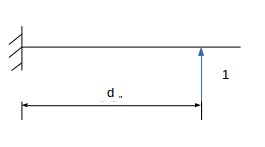
\includegraphics[width=0.6\linewidth]{images/dummy.png}
	\caption{Unit dummy system}
	\label{fig:dummy}
\end{figure}\\
The vertical displacement expression obtained through the Principle of Complementary Virtual Works is:
\begin{equation}
	u_d=\frac{S_PE_P\alpha T}{EJ}l_P(d-x_{CP})
\end{equation}
where $l_P$ is the length of the patch, $d$ the distance from the root of the point where the vertical displacement is computed, $x_{CP}$ is the center of the patch $x$-coordinate and $EJ$ is the bending stiffness of the structure, evaluated in the following way:
\begin{equation}
EJ=\frac{1}{12}[E_B(t_B^3+3t_Bt_P^2)b_B+E_P(t_P^3+3t_Pt_B^2)b_P]
\end{equation} 
where the $P$ subscript refers to the patch and $B$ to the beam substrate.\\
Therefore, all the results are consistent except for the ones obtained by the thermal analogy in OpenNastran95.


\subsection{Extension to Dynamics}
When it comes to dynamics, the scope is to minimize the difference between the actual response and the desired one. This can be done for the scaled aircraft in aeroelastic similarity in order to have the same modes and $flutter$ velocity of the reference one.\\
First of all, the problem needs to be re-casted into the state space form:\\
\begin{equation}
	M \ddot{u} +Ku=f_p ~ ~\text{Dynamic Equation}
\end{equation}\\
where
\begin{equation}
	f_p=[0...1...-1..0]^TS_pd_{31}\frac{V}{h}E_p
\end{equation}
is applied at the nodes where the patch is placed through a vector of zeros and ones.\\
The state space form will be:
	\[
	\begin{Bmatrix}
	\ddot{u}  \\ 
	\dot{u} 
	\end{Bmatrix}
	=\begin{bmatrix}
	0 & -MK^{-1}\\
	I & 0 \\
	\end{bmatrix}
	\begin{Bmatrix} 
	\dot{u}  \\ 
	u 
	\end{Bmatrix}+
	\begin{Bmatrix} 
	M^{-1}  \\ 
	O
	\end{Bmatrix}f_p
	\]
	
	\[
	u=
	\begin{bmatrix}
	0 & I
	\end{bmatrix}
	\begin{Bmatrix}
	\dot{u} \\
	u
	\end{Bmatrix}+
	\begin{bmatrix} 
	0
	\end{bmatrix}
	f_p
	\]
Since the scope is to minimize a parameter (the difference between the two dynamics), an \textit{Optimal Control} technique might be appropriate. As widely explained in \cite{c3}, the \textit{Optimal Control} problem is formulated as the minimization of a functional of this type:
\begin{equation}
f=\frac{1}{2}(x_f^TP_fx_f+\int_0^{t_f}(z^TW_{zz}z+u^TW_{uu}u)dt)
\end{equation}
This cost function is composed by the following contributes: the first term is the penalty applied to the final state $x_f$ through the weight matrix $P_f$. The second one weights the value attributed to the performance parameter $z$ during the time the control law is applied, the third one weights the control input signals $u$ to keep them limited also when the application is very demanding.
In this case, $u$ will be the PZT voltage while the performance parameter $z$ might be calculated using a \textit{Partial Implicit Model Following} (partial because it works with a subspace of the state, implicit since it uses the derivatives of the variables). This way, the difference between the actual and the desired dynamics can be minimized.
To sum up:\\
$y=Cx$ is a subspace of the state;\\
$\dot{y}=\hat{A}_dy=\hat{A}_dCx$ is the desired dynamics (the reference aircraft one);\\
$z=C\dot{x}-\dot{y}=[CA-\hat{A}_dC]x+CB_uu$ is therefore the performance parameter, where $A$ is the state matrix and $B_u$ the input matrix.\\
Once the cost function $f$ is completely defined, the problem of minimizing it can be reduced to the solution of the Continuous Algebraic Riccati Equation (CARE). The Kleinman's algorithm \cite{c4} is a method to solve it in a recursive manner. There is a Matlab built-in function called $are$ which implements it.


    
    
        

\section{Conclusions}
The main objective of this research was to find methods to model the piezoelectric actuator effect in OpenNastran95, where no elements of this type are available.\\
The first method, the thermal analogy, was already widespread in the bibliography concerning the smart structures modeling in MSC/Nastran. The other one, the applied bending moments modeling, is simply the output of a Virtual Work Principle applied to the sample problem. Having two different methods gives the possibility to compare results and validate the codes each other. And this is what has been done with MSC/Nastran. The difference in the results obtained with OpenNastran95 would require additional analyses. For example, it would be interesting to perform experimental tests on the piezoelectric actuators, in order to verify the simulation results.\\
As far as the Python code is concerned, the interest was to add new design variables (thickness and voltage) to perform the optimization of a scaled aircraft in aeroelastic similarity. This is linked to the Joan Mas Colomer's PhD thesis and I hope it can be helpful.\\
For sure, this work has been useful for me: it gave me the possibility to discover different softwares and to have a glance on what research is. Moreover, it helped me understanding what it means to collaborate with a research team: the capability of working autonomously without being afraid to ask for help when necessary.\\
I take this opportunity to thank Joan Mas Colomer and Joseph Morlier for their support and suggestions. 
    \clearpage

\footnotesize

\begin{thebibliography}{99} % Beamer does not support BibTeX so references must be inserted manually as below
	\bibitem[MathWorks, 2012-2015]{c1} MathWorks (2012-2015)
	\newblock Deflection of Piezoelectric Actuator,
	\newblock \emph{The Mathworks, Inc.} 
	\bibitem[Freed, Babuka, 1997]{c5}Brian D. Freed and Vit Babuka(1997)
	\newblock Finite Element Modeling of Composite Piezoelectric Structures with
	MSC/NASTRAN
	\newblock \emph{Smart Structures and Integrated Systems, (6 June 1997)}
	\bibitem[Reaves, Horta, 2003]{c2} Mercedes C. Reaves and Lucas G. Horta (2003)
	\newblock Piezoelectric Actuator Modeling Using
	MSC/NASTRAN and MATLAB,
	\newblock \emph{NASA/TM-2003-2 1265 1} 
	\bibitem[Stengel, 1993]{c3} Robert F. Stengel (1993)
	\newblock Optimal Control and Estimation
	\newblock \emph{Dover Publications, Inc.}
	\bibitem[Kleinman, 1968]{c4}D. Kleinman (1968)
	\newblock On an iterative technique for Riccati equation computations,
	\newblock \emph{IEEE Transactions on
		Automatic Control, vol. 13, pp 114-115}
\end{thebibliography}


\clearpage

\appendix
\onecolumn
\LARGE \textbf{Appendices}

\normalsize
\medskip
\textbf{Modeling through TEMP CARD}\\
The following OpenNastran95 input file computes displacements of the node set called $SET~5$. TEMP cards identify the locations at which thermal loads (voltage) is
applied.
\begin{verbatim}
ID    PZT CQUAD4 ELEMENTS 
APP   DISPLACEMENT                                                          
SOL   1,0
TIME  60                                                                                                                                       
CEND                                                                         
TITLE = Temperature PZT modeling
$ GLOBAL CASE
LABEL = CONSTRAINTS ARE - FIXED AND FREE ENDS.
SPC = 1 
TEMP(LOAD) = 1                                                                                                                                                                                        
$ Define set of elements for strain output
SET 4 =104
$ Define set of nodes for displacement output
SET 5 =325,335,345,355,365,375,385,395
OUTPUT                                                                  
DISP(PRINT) = 5
STRAIN = 4                                                
BEGIN BULK   
GRID,1,,0.00,0.00,0.00
GRID,2,,0.00,7.84,0.00
GRID,3,,0.00,15.68,0.00
GRID,4,,0.00,23.52,0.00
GRID,5,,0.00,31.36,0.00
...
GRID,447,,405.00,47.04,0.00
GRID,448,,405.00,54.88,0.00
GRID,449,,405.00,62.72,0.00
GRID,450,,405.00,70.56,0.00
CQUAD4,1,2,1,11,12,2
CQUAD4,2,2,2,12,13,3
CQUAD4,3,2,3,13,14,4
CQUAD4,4,2,4,14,15,5
...
CQUAD4,392,2,435,445,446,436
CQUAD4,393,2,436,446,447,437
CQUAD4,394,2,437,447,448,438
CQUAD4,395,2,438,448,449,439
CQUAD4,396,2,439,449,450,440 
$ Property card definition for aluminum 
$beam substrate
PCOMP,2,-5.08E-1,,,,,,,+PC1
+PC1,2,1.016,0.00000,YES
$ Property card definition for aluminum 
$beam substrate and piezoactuator lay-up
PCOMP,5,-5.08E-1,,,,,,,+PC5
+PC5,2,1.016,0.00000,YES,4,2.03E-1,0.0000,YES
$ Aluminum material properties
MAT1,2,7.2+4,,0.33333,2.758E-9,.0
$Piezo ceramic material properties, non-zero CTE
MAT1,4,6.9+4,,0.31000,7.700E-9,8.42-7 
PARAM,AUTOSPC,1 
SPC1,1,123456,1,THRU,10
TEMP,1,23,10.00,24,10.00,25,10.00
TEMP,1,26,10.00,27,10.00,28,10.00
TEMP,1,33,10.00,34,10.00,35,10.00
TEMP,1,36,10.00,37,10.00,38,10.00
TEMP,1,43,10.00,44,10.00,45,10.00
TEMP,1,46,10.00,47,10.00,48,10.00
TEMP,1,53,10.00,54,10.00,55,10.00
TEMP,1,56,10.00,57,10.00,58,10.00
TEMP,1,63,10.00,64,10.00,65,10.00
TEMP,1,66,10.00,67,10.00,68,10.00
TEMP,1,73,10.00,74,10.00,75,10.00
TEMP,1,76,10.00,77,10.00,78,10.00
TEMP,1,83,10.00,84,10.00,85,10.00
TEMP,1,86,10.00,87,10.00,88,10.00
TEMP,1,93,10.00,94,10.00,95,10.00
TEMP,1,96,10.00,97,10.00,98,10.00
TEMP,1,103,10.00,104,10.00,105,10.00
TEMP,1,106,10.00,107,10.00,108,10.00
TEMPD,1,0.0
ENDDATA
\end{verbatim}
\medskip
\textbf{Modeling through MOMENT CARD}\\
The following OpenNastran95 input file is set up to compute displacements of the node set called $SET~5$, modeling the actuation effect by mean of applied bending moments (card $MOMENT$).
\begin{verbatim}
	ID    PZT CQUAD4 ELEMENTS 
	APP   DISPLACEMENT                                                          
	SOL   1,0
	TIME  60                                                                                                                                       
	CEND                                                                         
	TITLE = Moment PZT modeling
	$ GLOBAL CASE
	LABEL = CONSTRAINTS ARE - FIXED AND FREE ENDS.
	SPC = 1                                                                      
	LOAD = 1                                                                                                                    
	$ Define set of elements for strain output
	SET 4 =104
	$ Define set of nodes for displacement output
	SET 5 =325,335,345,355,365,375,385,395
	OUTPUT                                                                  
	DISP(PRINT) = 5
	STRAIN = 4                                                
	BEGIN BULK   
	GRID,1,,0.00,0.00,0.00
	GRID,2,,0.00,7.84,0.00
	GRID,3,,0.00,15.68,0.00
	GRID,4,,0.00,23.52,0.00
	GRID,5,,0.00,31.36,0.00
	...
	GRID,447,,405.00,47.04,0.00
	GRID,448,,405.00,54.88,0.00
	GRID,449,,405.00,62.72,0.00
	GRID,450,,405.00,70.56,0.00
	CQUAD4,1,2,1,11,12,2
	CQUAD4,2,2,2,12,13,3
	CQUAD4,3,2,3,13,14,4
	CQUAD4,4,2,4,14,15,5
	...
	CQUAD4,392,2,435,445,446,436
	CQUAD4,393,2,436,446,447,437
	CQUAD4,394,2,437,447,448,438
	CQUAD4,395,2,438,448,449,439
	CQUAD4,396,2,439,449,450,440 
	$ Property card definition for aluminum 
	$beam substrate
	PCOMP,2,-5.08E-1,,,,,,,+PC1
	+PC1,2,1.016,0.00000,YES
	$ Property card definition for aluminum 
	$beam substrate and piezoactuator lay-up
	PCOMP,5,-5.08E-1,,,,,,,+PC5
	+PC5,2,1.016,0.00000,YES,4,2.03E-1,0.0000,YES
	$ Aluminum material properties
	MAT1,2,7.2+4,,0.33333,2.758E-9,.0
	$Piezo ceramic material (PZT-5A) properties
	MAT1,4,6.9+4,,0.31000,7.700E-9,0. 
	PARAM,AUTOSPC,1 
	SPC1,1,123456,1,THRU,10
	MOMENT,1,23,0,2.815E-1,.0,-1.,0.
	MOMENT,1,24,0,2.815E-1,.0,-2.,0.
	MOMENT,1,25,0,2.815E-1,.0,-2.,0.
	MOMENT,1,26,0,2.815E-1,.0,-2.,0.
	MOMENT,1,27,0,2.815E-1,.0,-2.,0.
	MOMENT,1,28,0,2.815E-1,.0,-1.,0.
	MOMENT,1,104,0,2.815E-1,.0,1.,0.
	MOMENT,1,105,0,2.815E-1,.0,2.,0.
	MOMENT,1,106,0,2.815E-1,.0,2.,0.
	MOMENT,1,107,0,2.815E-1,.0,2.,0.
	MOMENT,1,108,0,2.815E-1,.0,2.,0.
	MOMENT,1,109,0,2.815E-1,.0,1.,0.
	ENDDATA
\end{verbatim}
\medskip
\textbf{Input file template, to be filled with numerical values}\\
This Template needs to be filled with numerical values of materials properties, thicknesses and temperature loads. This is done by the $Python$ code reported afterwards. The rest of the data deck is identical to the ones above.
\begin{verbatim}
	$ Property card definition for aluminum beam substrate
	PCOMP,2,{z0},,,,,,,+PC1
	+PC1,2,{t1},0.00000,YES
	$ Property card definition for aluminum beam substrate and piezoactuator lay-up
	PCOMP,5,{z0},,,,,,,+PC5
	+PC5,2,{t1},0.00000,YES,4,{tp1},0.0000,YES
	$ Aluminum material properties
	MAT1,2,{E},,{nu},{rho_s},0.
	$Piezo ceramic material properties, non-zero CTE
	MAT1,4,{E_pzt},,{nu_pzt},{rho_pzt},{alpha}
	PARAM,AUTOSPC,1 
	SPC1,1,123456,1,THRU,10
	TEMP,1,23,{V1},24,{V1},25,{V1}
	TEMP,1,26,{V1},27,{V1},28,{V1}
	TEMP,1,33,{V1},34,{V1},35,{V1}
	TEMP,1,36,{V1},37,{V1},38,{V1}
	TEMP,1,43,{V1},44,{V1},45,{V1}
	TEMP,1,46,{V1},47,{V1},48,{V1}
	TEMP,1,53,{V1},54,{V1},55,{V1}
	TEMP,1,56,{V1},57,{V1},58,{V1}
	TEMP,1,63,{V1},64,{V1},65,{V1}
	TEMP,1,66,{V1},67,{V1},68,{V1}
	TEMP,1,73,{V1},74,{V1},75,{V1}
	TEMP,1,76,{V1},77,{V1},78,{V1}
	TEMP,1,83,{V1},84,{V1},85,{V1}
	TEMP,1,86,{V1},87,{V1},88,{V1}
	TEMP,1,93,{V1},94,{V1},95,{V1}
	TEMP,1,96,{V1},97,{V1},98,{V1}
	TEMP,1,103,{V1},104,{V1},105,{V1}
	TEMP,1,106,{V1},107,{V1},108,{V1}
	TEMPD,1,0.0
	ENDDATA
\end{verbatim}
\medskip
\textbf{Python code to fill the Nastran template input file}\\
Below, some parts of the Python code used to generate the OpenNastran95 input file for a static analysis. The template file reported above is filled with the values indicated in Python. This way, it is possible to use the PZT actuators thicknesses and voltages as design variables to perform the multidisciplinary optimization with the framework \textit{OpenMDAO}.
\begin{verbatim}
[...]
class NastranStatic(ExternalCode):
template_file = 'nastran_static_template.inp'
def __init__(self, node_id, node_id_all, n_stress, tn, tpn, mn, case_name):
super(NastranStatic, self).__init__()

#Identification number of the outer surface nodes
self.node_id = node_id

#Identification number of all the structural nodes
self.node_id_all = node_id_all

#Number of nodes on the outer surface
self.ns = len(node_id)

#Total number of structural nodes
self.ns_all = len(node_id_all)

#Number of stress outputs
self.n_stress = n_stress

#Number of regions where the thicknesses are defined
self.tn = tn

#Number of regions where the PZT thicknesses are defined
self.tpn = tpn
[...]
#Vector containing the thickness of each region
self.add_param('t', val=np.zeros(self.tn))

#Vector containing the offset of the bottom surf. from the reference plane
self.add_param('z0', val=np.zeros(self.tn))

#Vector containing the thickness of each PZT region
self.add_param('tp', val=np.zeros(self.tn))

#Vector containing the voltage of each patch
self.add_param('V', val=np.zeros(self.tn))
[...]
#Piezoelectric constant
self.add_param('d31', val=0)

#PZT Young's modulus
self.add_param('E_pzt', val=0)

#PZT Poisson's ratio
self.add_param('nu_pzt', val=0)

#PZT density
self.add_param('rho_pzt', val=0)

#Displacements of the nodes on the outer surface
self.add_output('u', val=np.zeros((self.ns, 3)))

#Von Mises stress of all elements
self.add_output('VMStress', val=np.zeros(self.n_stress))
[...]
def solve_nonlinear(self, params, unknowns, resids):

# Generate the input file for Nastran from the input file template and pressure values at the nodes
self.create_input_file(params)

# Parent solve_nonlinear function actually runs the external code
super(NastranStatic, self).solve_nonlinear(params, unknowns, resids)
output_data = self.get_output_data()

# Parse the output file from the external code and set the value of u
unknowns['u'] = output_data['u']

#Parse the output file from the external code and get the Von Mises Stresses
unknowns['VMStress'] = output_data['VMStress']

#Parse the output file from the external code and get the structural mass
unknowns['mass'] = output_data['mass']

def create_input_file(self, params):

f_node = params['f_node']
node_coord_all = params['node_coord_all']
t = params['t']
z0 = t/2.
m = params['m']
E = params['E']
nu = params['nu']
rho_s = params['rho_s']
tp = params['tp']
V = params['V']
d31 = params['d31']
E_pzt = params['E_pzt']
nu_pzt = params['nu_pzt']
rho_pzt = params['rho_pzt']

input_data = {}

#Assign each force value to its corresponding node ID in the input data dictionary
for i in range(len(f_node)):
input_data['Fx'+self.node_id[i]] = print_float_8(f_node[i, 0])
input_data['Fy'+self.node_id[i]] = print_float_8(f_node[i, 1])
input_data['Fz'+self.node_id[i]] = print_float_8(f_node[i, 2])
[...]
#Assign each thickness value to its corresponding ID in the input data dictionary
for i in range(len(t)):
input_data['t'+str(i+1)] = print_float_8(t[i])

#Assign each offset to its corresponding ID in the input data dictionary
for i in range(len(z0)):
input_data['z0'+str(i+1)] = print_float_8(z0[i])

#Assign each mass value to its corresponding ID in the input data dictionary
for i in range(len(m)):
input_data['m'+str(i+1)] = print_float_8(m[i])
[...]
#Assign the PZT Young's modulus to its input data dictionary key
input_data['E_pzt'] = print_float_8(E_pzt)

#Assign the PZT Poisson's ratio to its input data dictionary key
input_data['nu_pzt'] = print_float_8(nu_pzt)

#Assign the PZT density to its input data dictionary key
input_data['rho_pzt'] = print_float_8(rho_pzt)

#Assign the PZT constant to its input data dictionary key
input_data['d31'] = print_float_8(d31)

#Assign each PZT thickness value to its corresponding ID in the input data dictionary
for i in range(len(tp)):
input_data['tp'+str(i+1)] = print_float_8(tp[i])

#Assign each PZT voltage (temperature in nastran) to its corresponding ID in the input data dictionary
for i in range(len(V)):
input_data['V'+str(i+1)] = print_float_8(V[i])

#Read the input file template
f = open(self.template_file,'r')
tmp = f.read()
f.close()

#Replace the input data contained in the dictionary onto the new input file
new_file = tmp.format(**input_data)
inp = open(self.input_filepath,'w')
inp.write(new_file)
inp.close()

def get_output_data(self):
[...]
output_data = {}
output_data['u'] = u
output_data['VMStress'] = VMStress
output_data['mass'] = mass

return output_data
\end{verbatim}







\end{document}
